\subsection{Data Analysis Implementation}\label{sec:impl-data-analysis}
\subsubsection{Initial Dataset Analysis}
Initial analysis of the dataset constructed in section \ref{sec:impl-data-gatherer} revealed that it's comprised of 6547 rows spread across 67 columns, where each column corresponds to a feature. Out of the 67 columns, the vast majority is of numeric type, with only 5 being a text and 1, the prediction target column, referred to as \texttt{is\_bug} being of type boolean.

\subsubsection{Timestamps features transformation}\label{sec:impl-data-analysis:make-file-age}
As previously mentioned in section \ref{sec:data-available} the \timestamp{} and \prevTimestamp{} representing the time the current file commit was made as well as the last time commit has been made to the file had to be transformed into a single column outlining the age of the file - determining the staleness of it.
During the transformation, it has been discovered that in 7 instances the resulting column took on a negative value. This should have been impossible and as such, each case was investigated and verified against source data contained in Bitbucket server, as per section \ref{sec:data-available}. In all 7 cases, the actual data gathered from the Bitbucket server has been incorrect at the source. Given that short of manually gathering timestamps and correcting previous author data, there is no way to recover as well as the fact that such error occurred only in 7 records it was deemed best to removed them.
At the end of the transformation \timestamp{} and \prevTimestamp{} columns were removed, changing the shape of the dataset to 66 columns instead of initial 67.

\subsubsection{Files deleted}\label{sec:impl-data-analysis:files-deleted}
Progressively, an analysis of any missing values from all the columns was conducted. The first step was to determine if any of the files committed to having since been deleted. It has been determined by using the \files column provided by Sonar server. If the value of the column was not equal to 1 then such file no longer existed in the repository, despite the presence of historical code metrics. As a result, 431 rows were removed from the dataset. It should be noted that it doesn't mean that 431 different files were removed from the dataset as any file could have been committed to multiple times as each such commit would be represented by a row in the dataset. The obsolete file removal left the dataset at 6109 rows in 66 columns.

\subsubsection{Columns with all values at 0}\label{sec:impl-data-analysis:all-cols-at-0}
Next step was to check if there were any features present where all values were at 0 value. It has been determined that a column where all values are of 0 value would not contribute towards the prediction and therefore can be removed. The list of 19 removed columns is presented in Table \ref{tbl:zero-value-columns}. This step left the dataset with 6109 rows and 47 columns.

\begin{table}[!h]
\centering
\caption{Columns with all values at 0}
\label{tbl:zero-value-columns}
\begin{tabular}{@{}ll@{}}
\toprule
Column Name & Column Name \\ \midrule
blocker\_violations & public\_undocumented\_api \\
bugs & reliability\_remediation\_effort \\
confirmed\_issues & reopened\_issues \\
critical\_violations & security\_remediation\_effort \\
effort\_to\_reach\_maintainability\_rating\_a & skipped\_tests \\
false\_positive\_issues & test\_errors \\
generated\_lines & test\_failures \\
generated\_ncloc & vulnerabilities \\
it\_coverage & wont\_fix\_issue \\
it\_line\_coverage &  \\ \bottomrule
\end{tabular}
\end{table}



\subsubsection{Missing or negative values}\label{sec:impl-data-analysis:missing-or-negative-values}
Subsequently, an investigation into any values missing from any columns was investigated. The findings were summarized in Table \ref{tbl:missing-values-per-col}, with 13 columns showing a number of values missing. The missing values were then filled with the median per column, as per code listing \ref{code:missing-values-median-code}. Filling missing values with the median as opposed to mean metric has been preferred due to a large variance of some of the columns. In such instance it is more reliable to impute missing values from the median as mean is susceptible to extreme values - indicated by large variance values. It can be observed in Figure \ref{fig:high-variance} the variance distribution across columns - note that only columns with variance exceeding 100 have been included. Additionally, the \fileAgeInSec{} column has been removed as its variance value of approximately 0.5 billion would have skewed the graph making other properties unreadable. File age's variance is almost 17 times larger given that second largest variance of approximately 30000 belonging to \lines{} column.

\begin{code}
\captionof{listing}{Missing Values Filled per Column}
\label{code:missing-values-median-code}
\begin{minted}[breaklines]{python}
for col in cols:
        df[col] = df[col].fillna(df[col].median())
\end{minted}
\end{code}

\begin{figure}[!h]
    \centering
    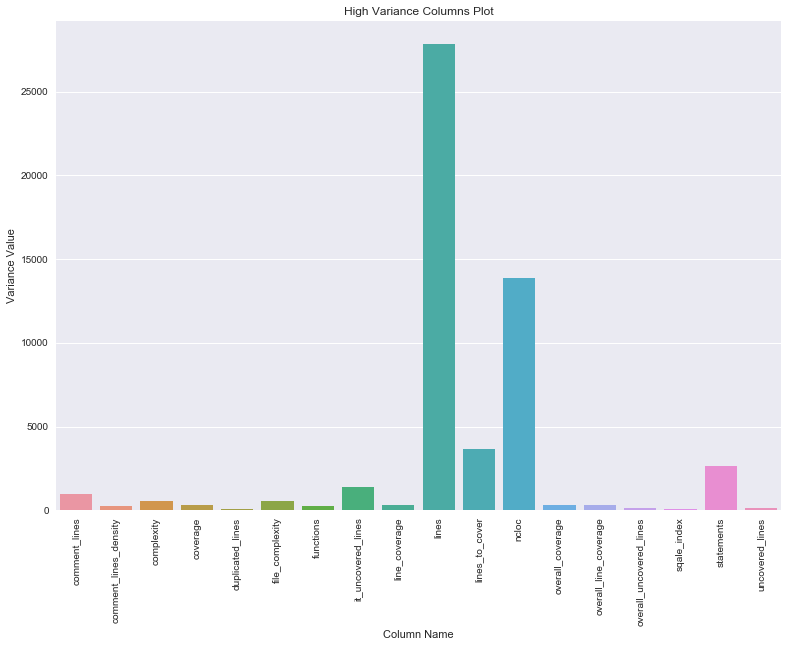
\includegraphics[scale=0.6]{\figpath/High_Variance_Columns_Plot.png}
    \caption{Attributes with high variance}
    \label{fig:high-variance}
\end{figure}

\begin{table}[!h]
\centering
\caption{Missing Values per Column}
\label{tbl:missing-values-per-col}
\begin{tabular}{@{}ll@{}}
\toprule
Column Name & No of missing values \\ \midrule
branch\_coverage & 2551 \\
coverage & 637 \\
function\_complexity & 119 \\
it\_uncovered\_lines & 3890 \\
line\_coverage & 637 \\
lines\_to\_cover & 637 \\
overall\_branch\_coverage & 2551 \\
overall\_coverage & 637 \\
overall\_line\_coverage & 637 \\
overall\_uncovered\_conditions & 2551 \\
overall\_uncovered\_lines & 637 \\
uncovered\_conditions & 2551 \\
uncovered\_lines & 637 \\ \bottomrule
\end{tabular}
\end{table}
\FloatBarrier

\subsubsection{Determining class balance} \label{sec:impl-data-analysis:class-balance}
Once the data has been cleaned and all missing values were filled, the next step was to determine the balance between values for the target class \isBug{}. It has been determined that the number of bug records was, 742, or approximately 12.15\% whereas non-bug records comprised of 5367, or approximately 87.85\%. As such the bug class was severely undersampled. Class balance has been conducted by checking how many rows in the dataset have had \texttt{True} value in the \isBug{} feature and how many were associated with \texttt{False} value. The reasoning behind not just subtracting the number of \texttt{True} labels from the total row count of the dataset were to catch any rows that had neither label associated with them. 

Given the steps undertaken it has been proven beyond doubt that all data samples have a value for \isBug{} feature, with data points categorized as \texttt{bug} being severely undersampled.

\subsubsection{Resampling the classes}\label{sec:impl-data-analysis:resampling}
Upsampling and downsampling techniques have both been investigated and implemented as part of the analysis. The downsampling method will randomly remove records from the majority class while the upsampling method will randomly duplicate minority class records in order to reach a balance between classes in the prediction target feature \isBug{}. 

In order for the process to be implemented first the determination into which class is in the majority and which is the minority had to be conducted. It has been implemented similarly to checking the class balance, however, instead of collecting values into lists by their indices, they are separated into 2 data frames, one for \texttt{True} and one for \texttt{False} classes. Then a determination into which of these data frames will be treated as majority and which is the representation of the minority class. At the end of the process data frames representing same is returned from the function for further processing.

Subsequently, the resampling of either class is conducted via \texttt{resample} function provided by sci-kit learn package. Said function takes in the following parameters:
\begin{itemize}
    \item data frame to be resampled. In the case of upsampling, it is the data frame containing all of the minority class records and in case of downsampling, it is the data frame representing the majority class.
    \item replace parameter takes in a boolean value. It is set to \texttt{True} for upsampling operation and \texttt{False} for the downsampling
    \item the number of records the minority or majority class needs to be resampled to. In case of sampling, this will be the number of records contained in the majority class and in case of downsampling it will match the number of records in the minority class data frame
    \item random state parameter - given that resampling operation is random by nature, the records are either randomly duplicated, upsampling, or deleted, downsampling, there is a need to ensure the same results between different executions of the complete analysis. That consistency is secured by providing the same number to the \texttt{random\_state} parameter. The value of the parameter is irrelevant, as long as it is provided.
\end{itemize}

In the last step data frames representing the majority and minority, now resampled, are combined into to form a single data frame representing the dataset and returned for further analysis.

\textbf{As a result of the resampling}, of the original data sample 2 datasets have been created. The upsampled dataset with 10734 of records and a downsampled dataset containing 1484 records.

\subsubsection{Data Correlation}\label{sec:impl-data-analysis:corr:generic-approach}
The following section will focus on identifying data correlation between features present in the dataset. The methods employed will be both numerical and visual. A numerical method has been employed for brevity and as verification for the visual method as it believed that with 40+ features it will be quite cumbersome to distinguish between high and low correlation values in a matrix.

\begin{figure}
    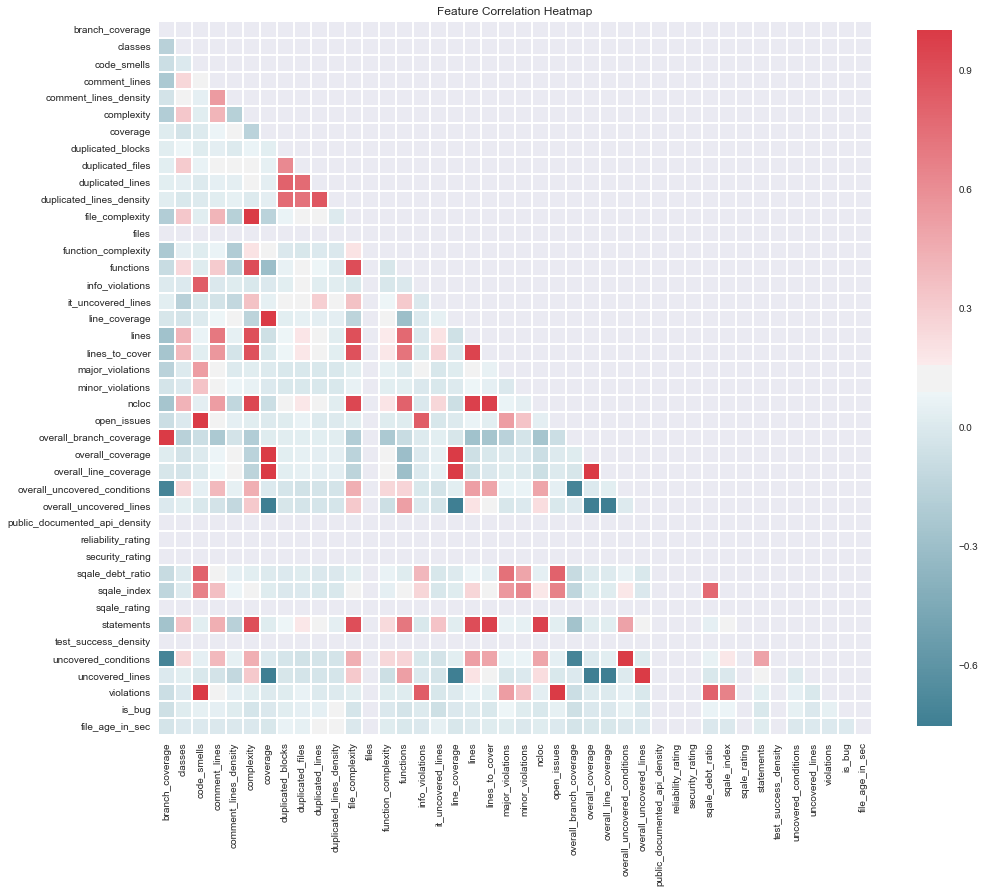
\includegraphics[scale=0.5,left]{\figCorrPath/Feature_Correlation_Heatmap.png}
    \caption{Feature Correlation Heatmap}
    \label{fig:correlation-all-features}
\end{figure}


The heatmap illustrated in Figure \ref{fig:correlation-all-features} served as a method of selecting candidates for:
\begin{itemize}
    \item feature transformation, where features with high positive correlation factor may be combined 
    \item selecting candidates from non-correlated features for visualizing how their values change in relation to one another
\end{itemize}

Unfortunately, the same figure was too large and involved to determine likely candidates visually, therefore it was decided to break it up into a number of smaller, subsection graphs. Features for the subsection graphs were selected based on name similarity or, based on previously acquired domain, similar metrics.
Therefore the most approach decided on was to split the correlation heatmap into subplots containing similar metrics, which was expected to produce a number of candidates for feature transformation. In order to decide how to transform feature candidates listed the following steps were undertaken in all cases:
\begin{enumerate}
    \item scatter plot depicting the relationship between the candidates
    \item the distribution of values 
    \item deciding on transformation approach, e.g. deletion, combination, etc
\end{enumerate}

Each heatmap was generated using the same implementation, as per code snippet \ref{code:corr-heatmap-impl} utilizing output of correlation function provided by Pandas DataFrame via \texttt{df.corr()} function. Said function provides a numerical metric of correlation between the attributes provided in the data frame. Should the value be positive then a positive correlation is present, meaning that an increase in one value will result in an increase, not necessarily of the same magnitude, in the corresponding metric. The opposite is true for metrics where the correlation factor is negative. The absolute value of the correlation factor represents the strength of the correlation with the greater value indicating a stronger relationship. Correlation factor near 0 is indicative of independence between attributes.

Each scatter-plot between a pair of attributes has been implemented using code snippet \ref{code:line-scatter-plot-impl}, where the $x$ and $y$ parameters refer to feature names and \texttt{data} parameter is supplied with the data frame representing the complete dataset.

\begin{code}
\captionof{listing}{Scatter Plot Between 2 Features - Implementation}
\label{code:line-scatter-plot-impl}
\begin{minted}[breaklines]{python}
sb.lmplot(x=column1, y=column2, truncate=True, size=5, data=dataFrame)
\end{minted}
\end{code}

More complex scatterplots, those between multiple attributes have been implemented using excerpt \ref{code:feat-transf:scatterplot}, where \texttt{data} is the complete dataset, \texttt{vars} is an array of column names to be include in the graph, \texttt{diag\_kind} is the kind of the diagram to be generated, between kernel density estimation plot or a histogram.
\begin{code}
\captionof{listing}{Scatter Plot Between Multiple Features - Implementation}
\label{code:feat-transf:scatterplot}
\begin{minted}[breaklines]{python}
sb.pairplot(data=df, vars =[column1, column2, column3, column4], diag_kind = 'kde', size=3)
\end{minted}
\end{code}

The distribution of attributes under analysis has been plotted on a single plane in a graph and has been implemented as depicted in code snippet \ref{code:feat-transf:distribution-multiplot}. It should be noted that the code has not been made generic to accommodate a variable number of attributes and is only suited for depicting pairs of attributes. To accommodate multiple attributes 2 places would have to be updated: the number of colours in the \texttt{colours} array would have to correspond to the number of attributes under analysis. The names of available colours can be found in Seaborn library's documentation. The second modification would have had to be made to the number of \texttt{sb.distplot(....)} calls - one call should be made for each attribute distribution to be plotted.

Alternatively, an additional method for depicting the relationship between attributes on three-dimensional space has been devised as per snippet \ref{code:feat-transf:3d-graph-impl}.

\FloatBarrier

%%%%%%%%%%%%%%%%%%%%%%%%%%%%%%%%%%%%%%%%%%%%%%%%%%%%%%%%%%%%%%%%%%%%%%%%%%%%%%%%%%%%%%%%%%%%%%%%%%%%%%%%%%%%%%%
\paragraph{Code Coverage Related Metrics}\label{sec:impl-data-analysis:corr:code-coverage}
The first subplot to be analyzed was populated with features relating to code coverage metrics:
\begin{itemize}\label{lst:code-coverage-candidates}
    \item \branchCoverage{}
    \item \overallBranchCoverage{}
    \item \overallCoverage{}
    \item \overallLineCoverage{}
    \item \overallUncoveredConditions{}
    \item \overallUncoveredLines{}
    \item \coverage{}
    \item \lineCoverage{}
    \item \uncoveredConditions{}
    \item \uncoveredLines{}
\end{itemize}
and it's correlation statistics can be observed in Figure \ref{fig:correlation-coverage-metrics-subplot}. From the same graph, 4 candidates for feature transformation into a single feature due to high positive correlation with one another can be identified:
\begin{enumerate}\label{lst:corr-sub:code-coverage-transf-candidates}
    \item \overallBranchCoverage{} and \branchCoverage{}
    \item \overallUncoveredLines{} and \uncoveredLines{}
    \item \overallCoverage{}, \overallLineCoverage{}, \coverage{} and \lineCoverage{}
    \item \overallUncoveredConditions and \uncoveredConditions{}
\suspend{enumerate}

\begin{figure}[!h]
    \centering
    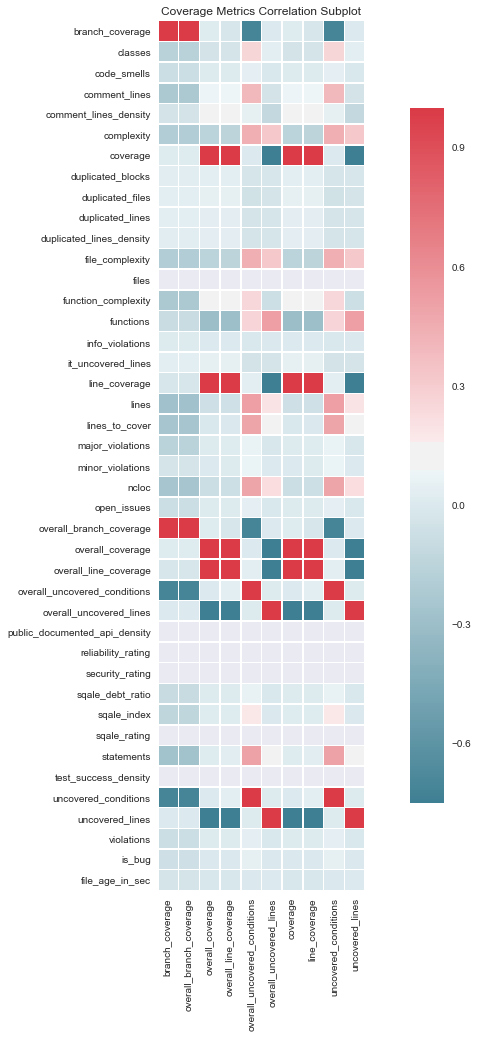
\includegraphics[scale=0.7]{\figCorrPath/Coverage_Metrics_Correlation_Subplot.png}
    \caption{Code Coverage Metrics Correlation Subplot}
    \label{fig:correlation-coverage-metrics-subplot}
\end{figure}
\FloatBarrier

Based on the scatter plot, generated from using code excerpt \ref{code:feat-transf:scatterplot}, depicted in Figure \ref{fig:candidate1-scatterplot} constructed for the transformation Candidate 1 listed above, it is thought that the attributes have a positive, almost perfectly linear relationship between one another, meaning that as one attribute increases in value so does the corresponding one, furthermore the increase or decrease in value is of the same magnitude.
\begin{figure}[!h]
    \centering
    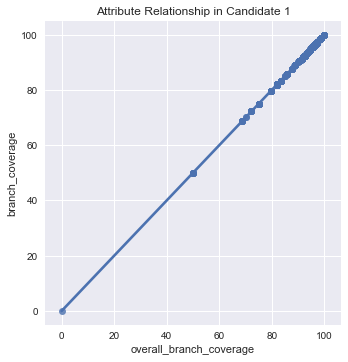
\includegraphics[scale=0.9]{\figCorrPath/Attribute_Relationship_in_Candidate_1.png}
    \caption{Relationship between \overallBranchCoverage{} and \branchCoverage{} attributes}
    \label{fig:candidate1-scatterplot}
\end{figure}

From the Figure \ref{fig:candidate1-distribution}, implemented by code snippet \ref{code:feat-transf:distribution-multiplot}, it can be surmised that the distribution of values for both attributes is perfectly aligned. To ascertain that claim an individual graph was plotted just for the invisible attribute \overallBranchCoverage{} which can be observed in Figure \ref{fig:candidate1-attrib2-distribution}.
From the investigation conducted it was deemed fair to conclude that it doesn't matter which attribute is preferred to be retained for Candidate 1 - \overallBranchCoverage{} or \branchCoverage{} as their values were almost identical. Based on the attribute name the column representing the overall coverage was selected to remain while the other was to be removed.

\begin{landscape}
\begin{figure}
\centering
\begin{minipage}{0.89\textwidth}
  \centering
  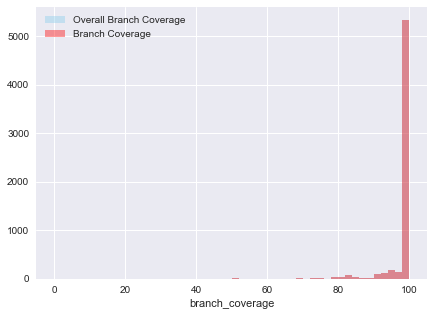
\includegraphics[scale=0.7]{\figCorrPath/Attribute_Distribution_in_Candidate_1.png}
    \caption{Distribution of \overallBranchCoverage{} and \branchCoverage{} attributes}
    \label{fig:candidate1-distribution}
\end{minipage}%
\begin{minipage}{0.89\textwidth}
   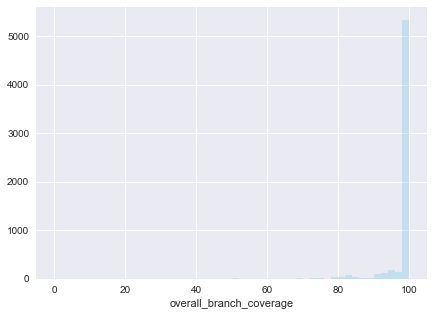
\includegraphics[scale=0.7]{\figCorrPath/Attribute_Distribution_in_overall_branch_coverage.png}
    \caption{Distribution of \overallBranchCoverage{} attribute}
    \label{fig:candidate1-attrib2-distribution}
\end{minipage}
\end{figure}
\end{landscape}
\FloatBarrier

Candidate 2 analysis started with the charting of a scatter plot for the selected attributes, the \overallUncoveredLines{} and \uncoveredLines{}, presented in Figure \ref{fig:candidate2-scatterplot}, and as with Candidate 1 displayed a positive linear relationship between the data points, with the majority of data focused close to 0 value.

\begin{figure}[!h]
    \centering
    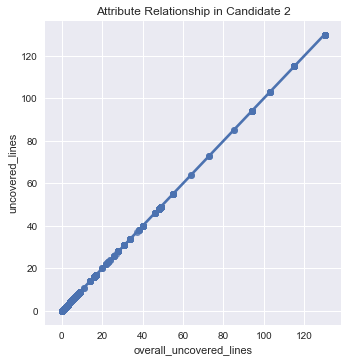
\includegraphics[scale=0.9]{\figCorrPath/Attribute_Relationship_in_Candidate_2.png}
    \caption{Relationship between \overallUncoveredLines{} and \uncoveredLines{} attributes}
    \label{fig:candidate2-scatterplot}
\end{figure}

The distribution of the \overallUncoveredLines{} and \uncoveredLines{} is the same as per Figure \ref{fig:candidate2-distribution}. Since it has been previously illustrated that when only 1 graph line is visible it is in fact perfectly overlain over the distribution line for the other attribute in the analysis of Candidate 1, therefore, a special graph depicting the distribution of \uncoveredLines{} will not be provided.
\begin{figure}
    \centering
  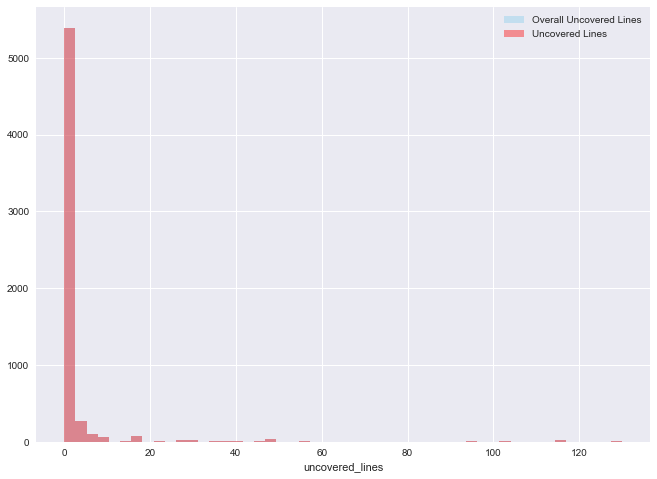
\includegraphics[scale=0.7]{\figCorrPath/Attribute_Distribution_in_Candidate_2.png}
    \caption{Distribution of \overallUncoveredLines{} and \uncoveredLines{} attributes}
    \label{fig:candidate2-distribution}
\end{figure}
In case of Candidate 2 it  has been decided to retain \overallUncoveredLines{} attribute as using domain knowledge of the metrics it stood to reason that this attribute would be more encompassing than \uncoveredLines{}.
\FloatBarrier

Given the depiction of both the linear relationship between the multiple  attributes of \overallCoverage{}, \overallLineCoverage{},\coverage{} and \lineCoverage{}, presented in Figure \ref{fig:candidate3-pairplot} and the distribution, provide on the diagonal it was summarily concluded that the attributes follow the same trends and only one of the four should be retained. Therefore, based on previous domain knowledge of the metrics \overallCoverage{} was deemed the most encompassing and has been retained.
% \todo{the pair plot needs an update of the title as it's not distribution. Plus need to plot distributions as pair plot diagonal is NOT a representation of distribution}
\begin{figure}[!h]
    \centering
    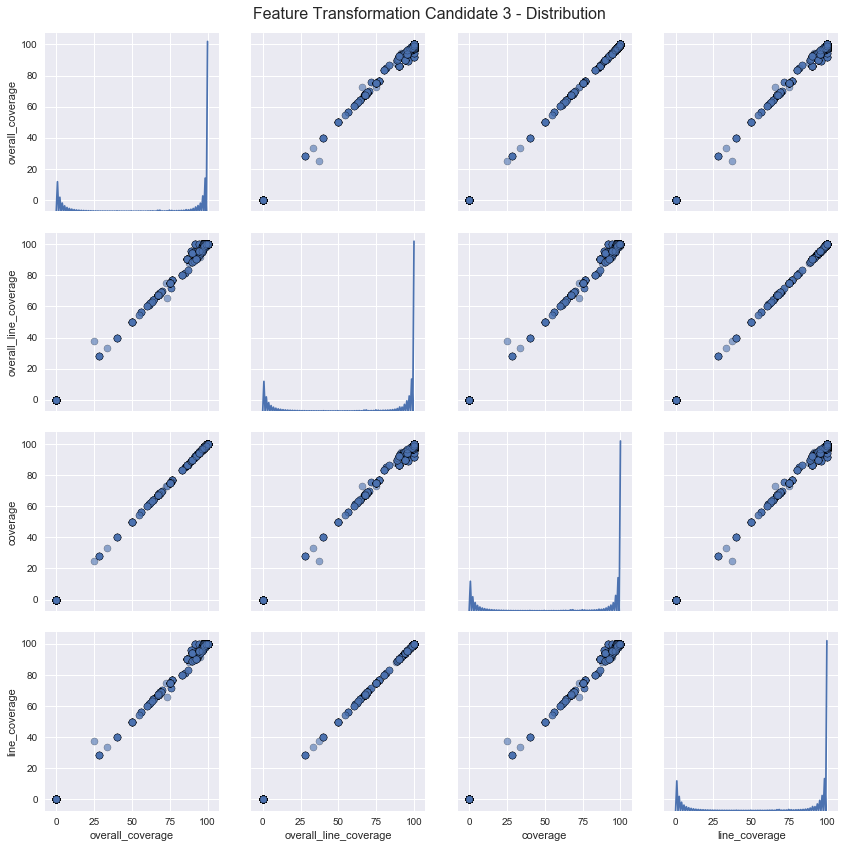
\includegraphics[scale=0.5]{\figCorrPath/Attribute_Relationship_in_Candidate_3.png}
    \caption{Relationship between multiple attributes}
    \label{fig:candidate3-pairplot}
\end{figure}

\FloatBarrier

The last feature transformation will be conducted between \overallUncoveredConditions{} and \uncoveredConditions{} attributes. In Figure \ref{fig:candidate4-scatterplot} it can be observed a perfectly linear relationship between the two attributes under investigation. Additionally, a change in one attribute corresponds directly to an increase of the corresponding attribute not only in the direction of the change but also in the magnitude. Furthermore, from Figure \ref{fig:candidate4-distribution} again a perfectly aligned distribution of both attributes can be observed leading to a conclusion that the attributes under question are equivalent.

\begin{figure}[!h]
    \centering
    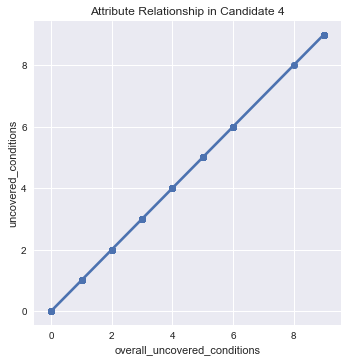
\includegraphics[scale=0.7]{\figCorrPath/Attribute_Relationship_in_Candidate_4.png}
    \caption{Relationship between \overallUncoveredConditions{} and \uncoveredConditions{} attributes}
    \label{fig:candidate4-scatterplot}
\end{figure}

\begin{figure}[!h]
    \centering
    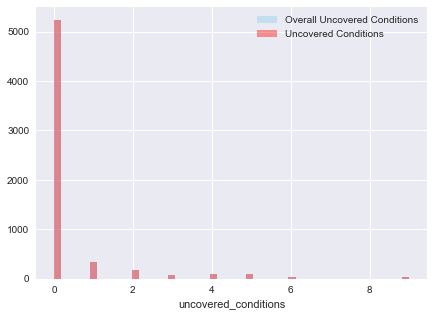
\includegraphics{\figCorrPath/Attribute_Distribution_in_Candidate_4.png}
    \caption{Distribution of \overallUncoveredConditions{} and \uncoveredConditions{} attributes}
    \label{fig:candidate4-distribution}
\end{figure}

\FloatBarrier
%%%%%%%%%%%%%%%%%%%%%%%%%5
\textbf{In conclusion} all features investigated in this section have displayed high positive relationship with one another, very strong linear relationship as well as almost perfectly aligned data distribution. Therefore, only 4 of the 10 attributes, enumerated in section \ref{lst:code-coverage-candidates}, have been retained:

\begin{itemize}
    \item \overallBranchCoverage{}
    \item \overallUncoveredLines{}
    \item \overallCoverage{}
    \item \overallUncoveredConditions{}
\end{itemize}

\paragraph{Line and complexity features}\label{sec:impl-data-analysis:corr:line-and-complexity}
In the following section, a number off attributes will be investigated with regards to the possibility of transforming said features and reducing the dimensionality of the overall dataset. Given a subplot of a heatmap presented in Figure \ref{fig:correlation-line-metrics-subplot} the attributes under analysis are, based on their high correlation:
\resume{enumerate}
    \item \complexity{}, \fileComplexity{}    \item \statements{}, \linesToCover{}
    \item \ncloc{}, \lines{}
\suspend{enumerate}
It is worth noting that despite similar naming \functionComplexity{} metric does not display a strong correlation with the other two complexity metrics and was not included  as part of Candidate 5.

The numbering of feature transformation candidates is being continued from the previous section, where candidates 1 through 4 were discussed.

Starting with Candidate 5, in Figure \ref{fig:candidate5-pairplot}, it can be observed that \complexity{} and \fileComplexity{} have an outstandingly well defined linear relationship. The attribute distribution also follows the same pattern, with a highly pronounced left tail. 

\begin{figure}
    \centering
    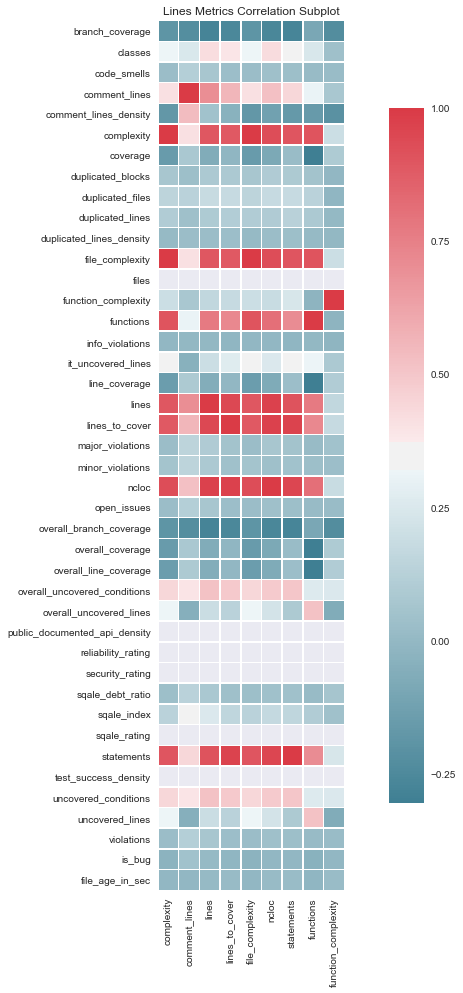
\includegraphics[scale=0.7]{\figCorrPath/Lines_Metrics_Correlation_Subplot.png}
    \caption{Line Metrics Correlation Subplot}
    \label{fig:correlation-line-metrics-subplot}
\end{figure}

\begin{figure}[!h]
    \centering
    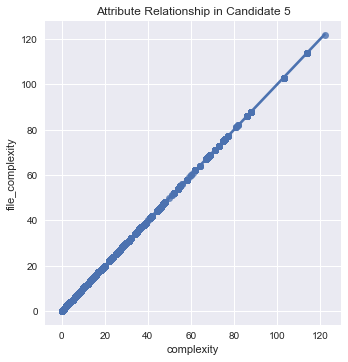
\includegraphics[scale=0.7]{Figures/correlation/Attribute_Relationship_in_Candidate_5.png}
    \caption{Relationship between \complexity{} and \fileComplexity{} attributes}
    \label{fig:candidate5-pairplot}
\end{figure}

\begin{figure}[!h]
    \centering
    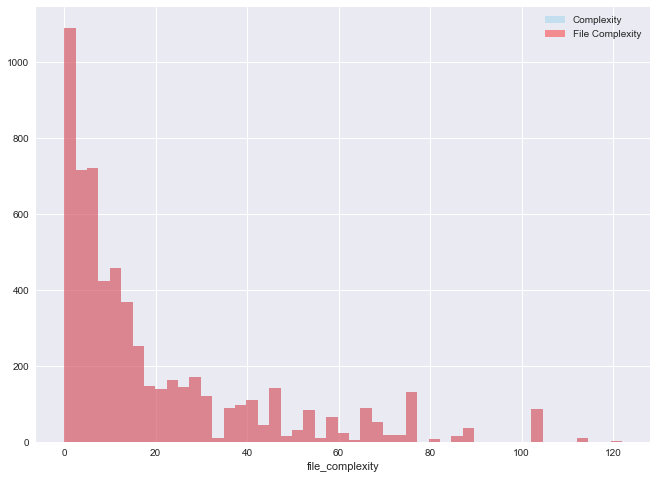
\includegraphics[scale=0.6]{Figures/correlation/Attribute_Distribution_in_Candidate_5.png}
    \caption{Distribution of \complexity{} and \fileComplexity{} Attributes}
    \label{fig:candidate5-distribution}
\end{figure}

For Candidate 6, \statements{} and \linesToCover{}, displayed in Figure \ref{fig:candidate6-scatterplot}, the relationship between them is again distinctly linear, while the distribution, as per Figure \ref{fig:candidate6-distribution} is similar with again a pronounced left tail. 

\begin{figure}[!h]
    \centering
    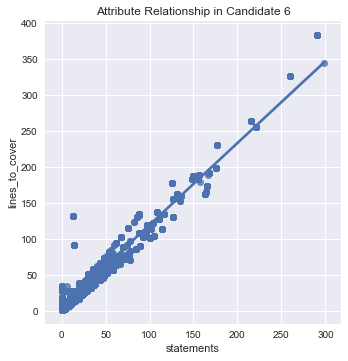
\includegraphics[scale=0.7]{Figures/correlation/Attribute_Relationship_in_Candidate_6.png}
    \caption{Relationship between \statements{} and \linesToCover{} Attributes}
    \label{fig:candidate6-scatterplot}
\end{figure}

\begin{figure}
    \centering
    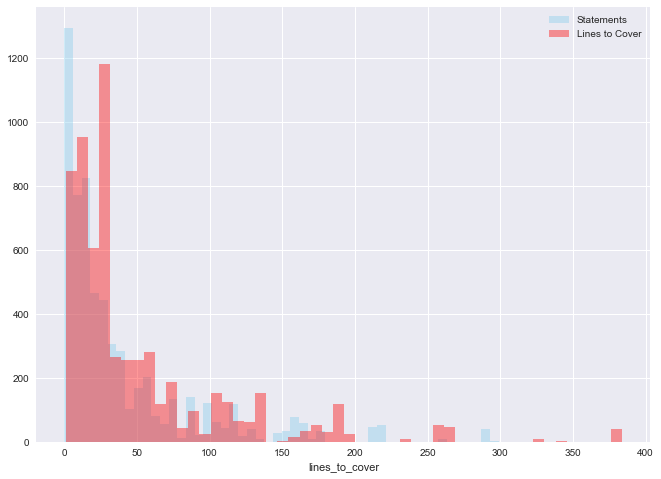
\includegraphics[scale=0.6]{Figures/correlation/Attribute_Distribution_in_Candidate_6.png}
    \caption{Distribution of \statements{} and \linesToCover{} Attributes}
    \label{fig:candidate6-distribution}
\end{figure}

In the next feature transformation candidate, numbered seventh, the relationship between \ncloc{} and \lines{} attributes is again quite linear, as per Figure \ref{fig:candidate7-scatterplot}. From the distribution of the attributes, displayed in Figure \ref{fig:candidate7-distribution} it can be concluded that they follow the distinctly similar pattern.

\begin{figure}
    \centering
    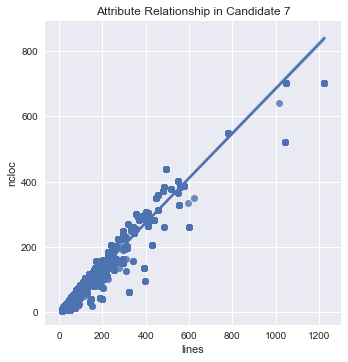
\includegraphics[scale=0.7]{Figures/correlation/Attribute_Relationship_in_Candidate_7.png}
    \caption{Relationship between \ncloc{} and \lines{} Attributes}
    \label{fig:candidate7-scatterplot}
\end{figure}

\begin{figure}
    \centering
    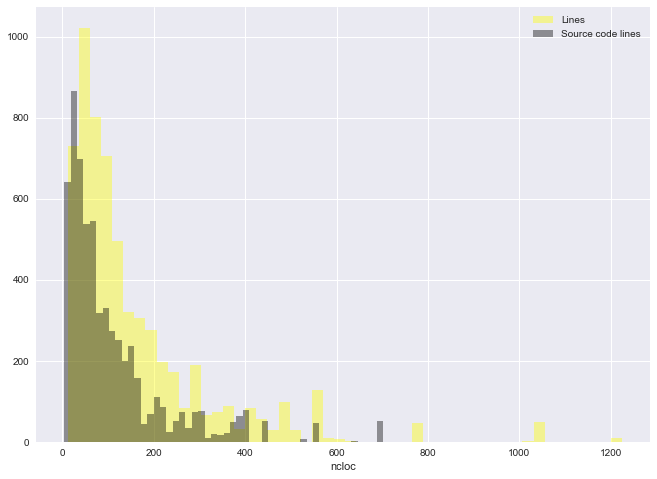
\includegraphics[scale=0.6]{Figures/correlation/Attribute_Distribution_in_Candidate_7.png}
    \caption{Distribution of \ncloc{} and \lines{} Attributes}
    \label{fig:candidate7-distribution}
\end{figure}


In order to further the analysis of the candidates, given the high correlation between a number of features, a number of three-dimensional plots were developed. They serve to better illustrate the relationship between multiple attributes at a time than multiple two-dimensional plots.

From Figure \ref{fig:3d:ncloc-linesToCover-statements} it can be observed that there is an almost perfect linear relationship between \statements{}, \ncloc{} and \lines{} attributes- and this stands to reason as all three metrics would be used to describe source code, with the distinction of \lines{} attribute covering both comment and source code lines in any file. This relationship can also be viewed in Figure \ref{fig:3d:statements-lines-commentLines}, where it can be observed that the higher the number of lines the higher the number of both \statements{} and \commentLines{}. The divergence of a small portion of \lines{} attribute from the main graph line is attributed to a growing number of comment lines in the code as opposed to source ones, as covered by \statements{}. This divergence points to different regression lines for \lines{} vs\commentLines{} as well as \lines{} and \statements{}, therefore those 3 are not equivalent and will not be folded up into a single metric.
\begin{figure}[!h]
    \centering
    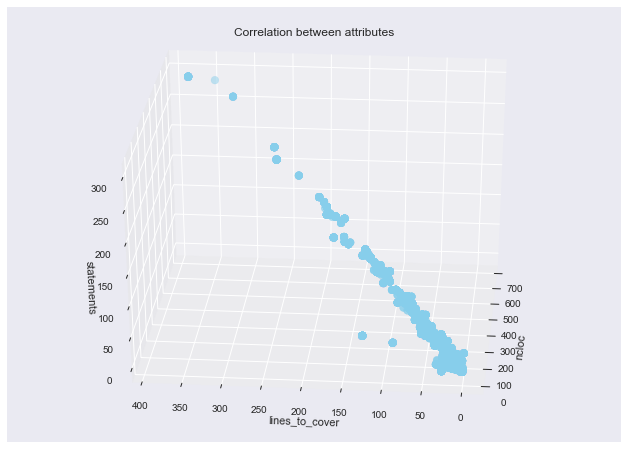
\includegraphics[scale=0.65]{Figures/three-d/Correlation-between-attributes-ncloc-lines_to_cover-statements.png}
    \caption{Relationship between multiple attributes}
    \label{fig:3d:ncloc-linesToCover-statements}
\end{figure}

\begin{figure}[!h]
    \centering
    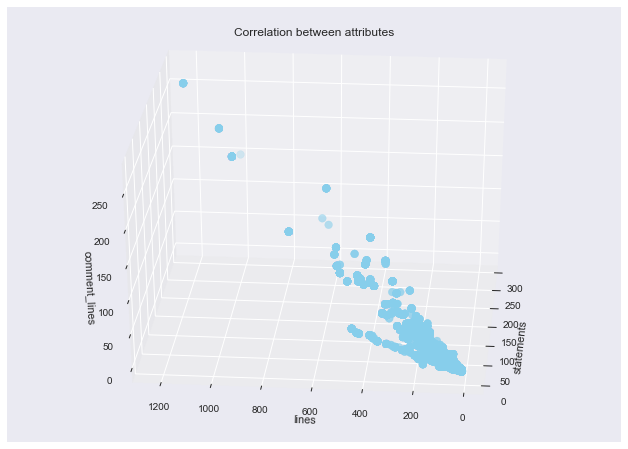
\includegraphics[scale=0.65]{Figures/three-d/Correlation-between-attributes-statements-lines-comment_lines.png}
    \caption{Relationship between multiple attributes}
    \label{fig:3d:statements-lines-commentLines}
\end{figure}

In the exploration of the trends, a plot depicting the relationship between \lines{}, \fileComplexity{} and \commentLines{} has been devised, as it is commonly thought that the more complex the code the more lines of comments and other documentation should be encountered. The results can be seen in Figure \ref{fig:3d:fileComplexity-lines-commentLines} and from the dataset gathered it looks that the hypothesis holds true, there is a correlation between the complexity of a file, its size in absolute terms - represented in the \lines{} attribute, and the number of comments in a given file. 
However, while the trend is present, those metrics are not equivalent and it has been decided against combining them into a single metric.
\begin{figure}[!h]
    \centering
    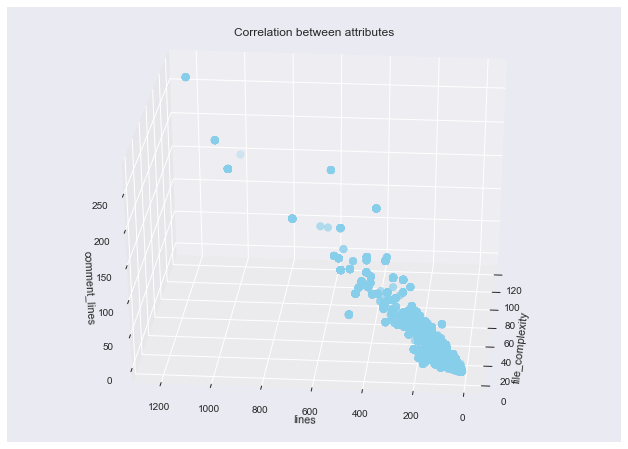
\includegraphics[scale=0.65]{Figures/three-d/Correlation-between-attributes-file_complexity-lines-comment_lines.png}
    \caption{Relationship between multiple attributes}
    \label{fig:3d:fileComplexity-lines-commentLines}
\end{figure}

\FloatBarrier
\textbf{In Conclusion} from the features listed at the beginning of this section it has been sufficiently determined that the following pairs can be safely transformed into a single feature:
\begin{itemize}
    \item \complexity{} and \fileComplexity{} - linear relationship and similar looking distribution
    \item \statements{} and \linesToCover{} - linear relationship and approximately the same distribution
    \item \lines{} and \ncloc{} quite a linear relationship, similar distribution between all.
\end{itemize}

The \complexity{}, \linesToCover{} and \ncloc{} have been retained while their corresponding pairs have been removed from further analysis.
\FloatBarrier
%%%%%%%%%%%%%%%%%%%%%%%%%%%%%%%%%%%%%%%%%%%%%%%%%%%%%%%%%%%%%%%%%%%%%%%%%%%%%%%%%%%%%%%%%%%%%%%%%
\paragraph{Sonar Violation Metrics}\label{sec:impl-data-analysis:corr:sonar-violations}
\begin{figure}[!h]
    \centering
    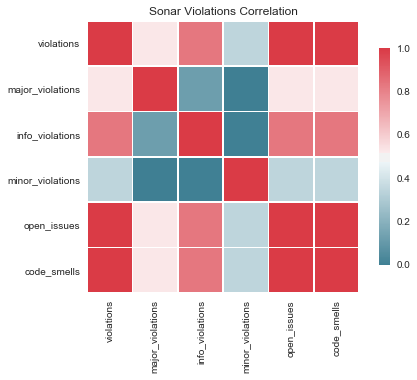
\includegraphics[scale=0.7]{Figures/correlation/Sonar_Violations_Correlation.png}
    \caption{Sonar Violation Metrics Correlation Subplot}
    \label{fig:correlation-sonar-violation-metrics-subplot}
\end{figure}

The following section will investigate if the following candidates can be transformed as per Figure \ref{fig:correlation-sonar-violation-metrics-subplot} there is a strong positive correlation between them:
\resume{enumerate}
    \item \openIssues{}, \violations{} and \codeSmells{}
    \item \majorViolations{}, \minorViolations{} and \infoViolations{}
\suspend{enumerate}

Starting with Candidate 8, the relationship between the attributes appears to be a strong linear one, as can be observed in Figure \ref{fig:3d:candidate8-relationship}. Unfortunately, despite the indications of a strong relationship, there aren't enough data points available to prove it beyond any doubt. The distribution graph, in Figure \ref{fig:candidate8-distribution}, however, clearly states that the distribution of whatever little data points that are available matches perfectly between the three attributes.

\begin{figure}
    \centering
    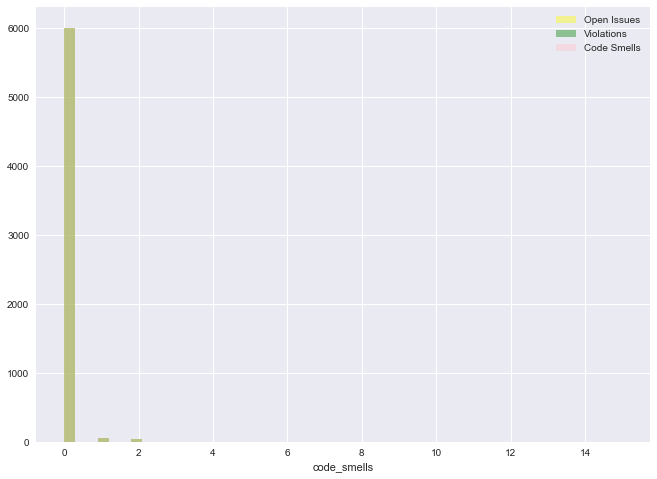
\includegraphics[scale=0.6]{Figures/correlation/Attribute_Distribution_in_Candidate_8.png}
    \caption{Distribution of attributes in Candidate 8}
    \label{fig:candidate8-distribution}
\end{figure}

\begin{figure}[!h]
    \centering
    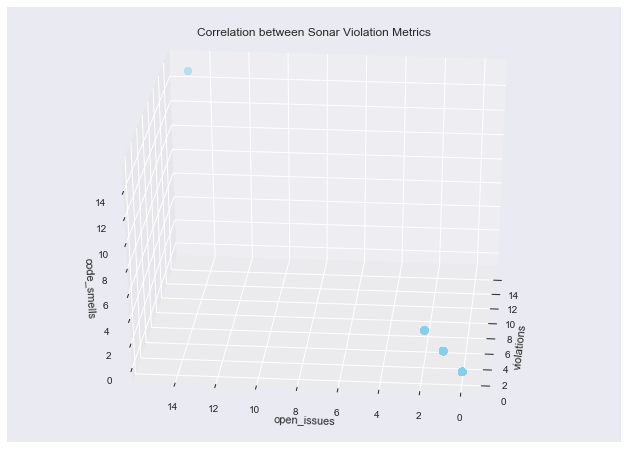
\includegraphics[scale=0.6]{Figures/three-d/Correlation_between_attributes_violations_open_issues_code_smells.png}
    \caption{Correlation between Sonar violation attributes}
    \label{fig:3d:candidate8-relationship}
\end{figure}

\begin{figure}[!h]
    \centering
    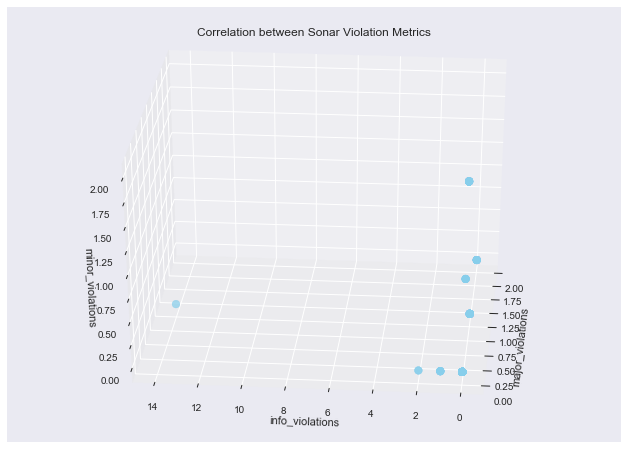
\includegraphics[scale=0.6]{Figures/three-d/Correlation_between_attributes_major_violations_info_violations_minor_violations.png}
    \caption{Correlation between Sonar violation attributes}
    \label{fig:3d:candidate9-relationship}
\end{figure}

\begin{figure}
    \centering
    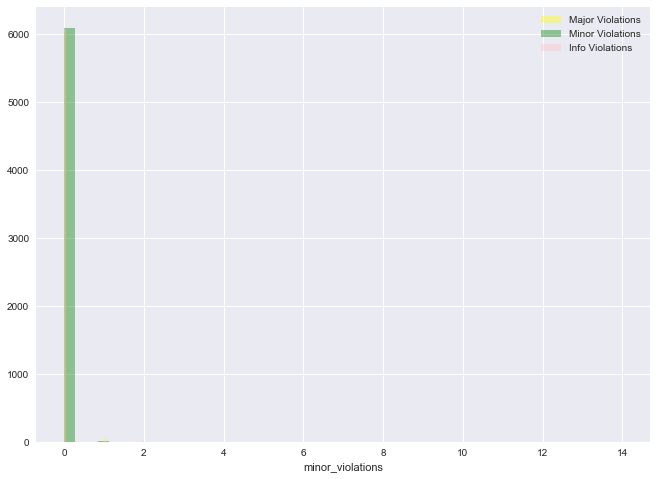
\includegraphics[scale=0.6]{Figures/correlation/Attribute_Distribution_in_Candidate_9.png}
    \caption{Distribution of attributes in candidate 9}
    \label{fig:candidate9-distribution}
\end{figure}

\textbf{In conclusion} the \openIssues{}, \codeSmells{} and \violations{} features can be transformed into a single feature as they show an indication of a linear relationship and have an identical distribution. As such \violations{} feature will be retained while the other 2 will be dropped from the analysis.

A conclusion with regards to remaining metrics is that no strong opportunity for transformation presented itself as there is little defined relationship between the attributes. Furthermore, based on domain knowledge of \infoViolations{}, \minorViolations{} and \majorViolations{} it is concluded that those metrics are independent of one another. 

However, when drawing from the domain knowledge of Sonar metrics, \violations{} is an all-encompassing term used for describing any infraction against rules defined as part of the analysis, such as that depicted by \infoViolations{}, \minorViolations{} or \majorViolations{}. As such, it is natural that \violations{} attribute will be closely related to those metrics. Therefore, the only violation describing metric retained will be \violations{}.
% \FloatBarrier

\paragraph{Code Duplication Metrics}\label{sec:impl-data-analysis:corr:code-duplication}

\begin{figure}
    \centering
    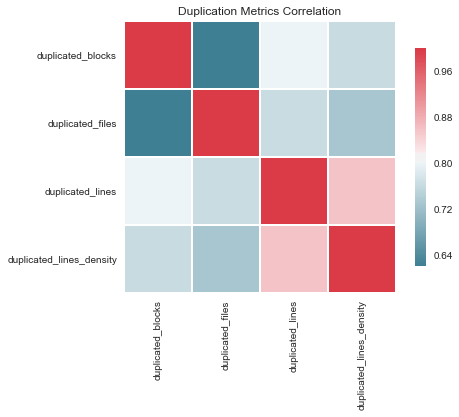
\includegraphics[scale=0.75]{Figures/correlation/Duplication_Metrics_Correlation.png}
    \caption{Code Duplication Metrics Correlation Subplot}
    \label{fig:correlation-code-duplication-metrics-subplot}
\end{figure}

Based on the correlation graph for code duplication metrics the following candidate has been chosen for the analysis:
\resume{enumerate}
    \item \duplicatedBlocks{}, \duplicatedFiles{}, \duplicatedLines{} and \duplicatedLinesDensity{}
\end{enumerate}

\begin{figure}
    \centering
    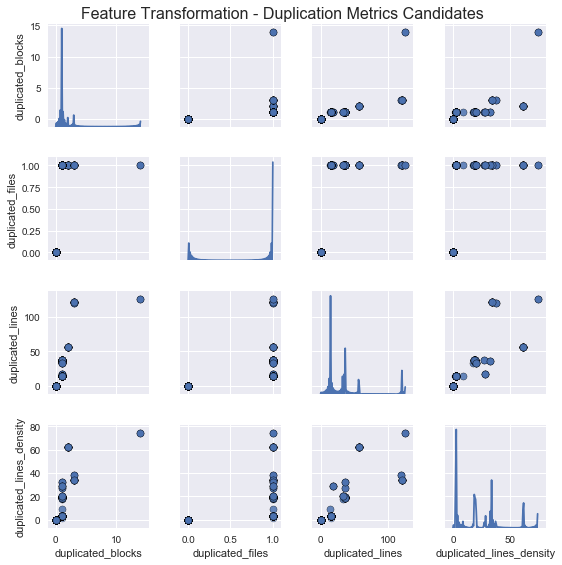
\includegraphics[scale=0.75]{Figures/correlation/Attribute_Relationship_in_Duplication_Metrics.png}
    \caption{Relationship between multiple attributes}
    \label{fig:candidate10-distribution}
\end{figure}


\textbf{In conclusion} no strong opportunity for transformation has been found between code duplication metrics as the correlation appears to be of small magnitude. The only exception has been displayed by \duplicatedBlocks{} and \duplicatedFiles{} features that showed a strong negative correlation.
\FloatBarrier
